\newpage
\section{Detailed Background and Theory}
\subsection{From Feynman to the linear optical quantum computer}
It was Richard Feynman in 1982 who first imagined it might be possible to efficiently simulate quantum systems with other quantum systems and hence end up doing computations that no classical computer could do in a reasonable (polynomial) time. Since then the theory has come a long way and there are many diverse research efforts trying to realise his idea. The work in this report is motivated by a particular paradigm called the linear optical quantum computer LOQC or often called the KLM protocol \cite{knill_efficient_2000}, this requires only standard optical elements to be able to fully simulate a quantum computer. This is inline with the five requirements set out by DiVincenzo in 1998 \cite{divincenzo_quantum_1998} for a full quantum computer.
\begin{itemize}
	\item A scalable physical system with well characterized
qubits
	\item The ability to initialize the state of the qubits to a
simple fiducial state, such as $\ket{000...}$
	\item Long relevant decoherence times, much longer than
the gate operation time
	\item A “universal” set of quantum gates
	\item A qubit-specific measurement capability
\end{itemize}



\begingroup
    \centering  
    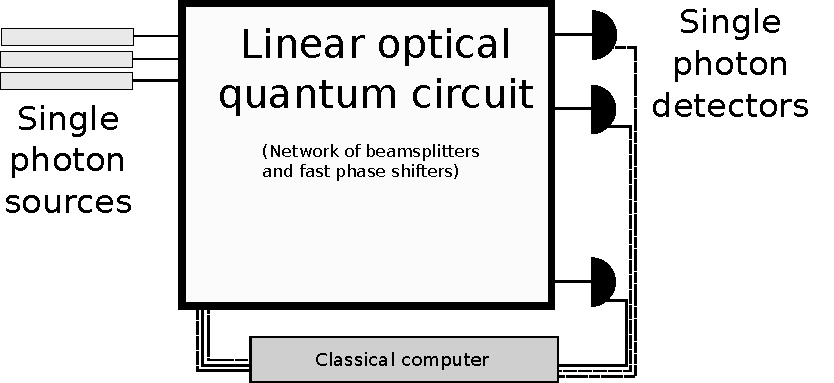
\includegraphics[width=18cm]{img/theory/loqc.pdf}
    \captionof{figure}{A conceptual outline of the architecture of a LOQC, single photon sources supply the qubits which are fed into reconfigurable circuits which are altered depending on the pattern of photons detected at the detectors. }
     \vspace{3pt} \label{loqc}
\endgroup



We focus in on the first criteria from DiVencenzo \cite{divincenzo_physical_2000}, "A scalable system with well characterized qubits", in the context of figure \ref{loqc} this refers to the single photon sources, we require them to be indistinguishable from each other so that the quantum interference which happens in the circuit can be of high visibility. 



\subsection{From bulk optics to integrated silicon photonics}
Quantum optics experiments were first conducted in bulk optics \cite{burnham_observation_1970} and since then they have allowed for the development of a large body of physics. Such experiments have certain basic elements in common such as beam splitters, filters, polarisation controllers, phase shifters, etc. With these elements occupying a fair amount of space in a lab there is a practical size limit on what can be done, hence there has been a recent push into compressing such optical experiments onto a single chip. Each of the optical elements described previously can be implemented onto such chips. The free space propagation of light is replaced by waveguides etched onto materials such as silicon, lithium niobate or glass. Beam splitters and couplers are implemented by running two waveguides close enough to each other so that light can couple between them via their evanescent fields. Filters are implemented as ring resonators which are circular cavaties with which only certain wavelengths of light will resonate and hence be filtered. Phase shifts can be induced by heating small portions of the chip with an electrical probe.

Here we focus in on a particular element, the ring resonator on silicon photonic devices. Silicon is an attractive material primarily due to the already established microchip industry which can produce highly precise structures at the nanoscale on the back of decades of demand for faster and smaller computing devices. Furthermore silicon has a high $\chi^{(3)}$ non-linearity enabling frequency conversion and hence the implementation of a single photon source.

\subsection{Ring Resonators}
Ring resonators are used as single photon sources. However to understand their behaviour to first order no quantum mechanics is needed. Here are the 3 governing equations:
%Need to talk about how ring resonators shape this stuff

SPLIT RESONANCES

\begingroup
    \centering  
    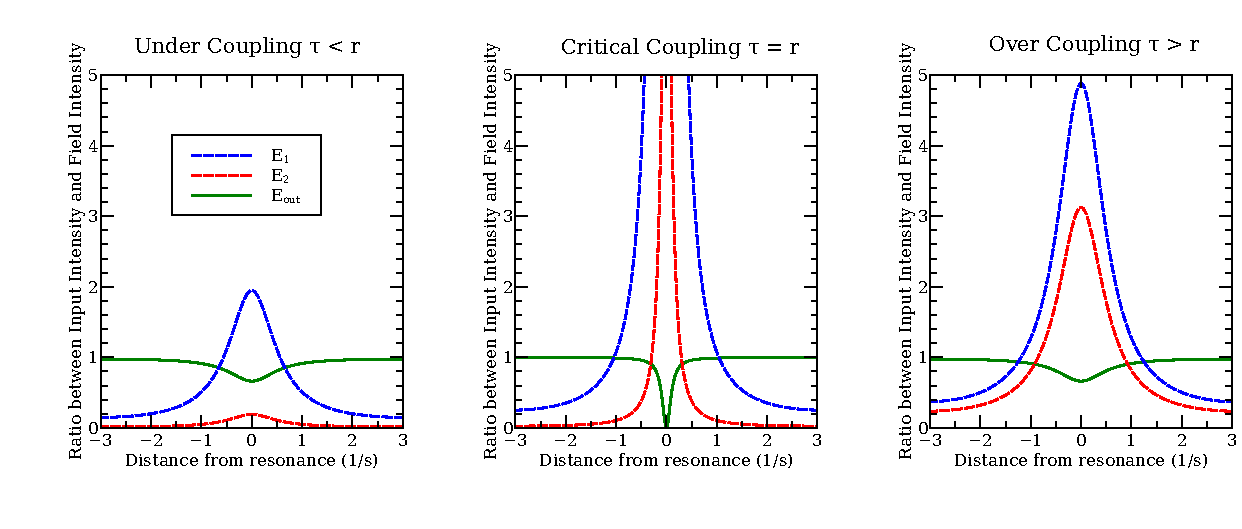
\includegraphics[width=18cm]{img/theory/coupling.pdf}
    \captionof{figure}{Notice how similar under and over coupling are to each other}
     \vspace{3pt} \label{crossCompare}
\endgroup

\begingroup
\centering
    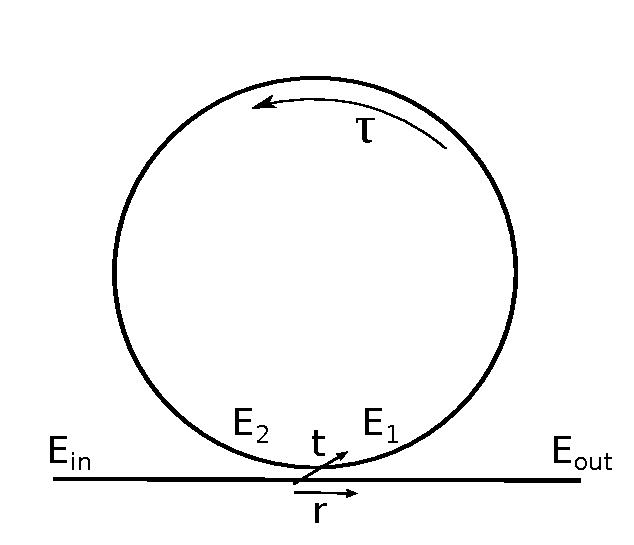
\includegraphics[width=5cm]{img/theory/ring.pdf}
\captionof{figure}{ahhh}
\endgroup
\begin{equation}
\left |\frac{E_{out}}{E_{0}}\right|^2=\frac{r^2-2r\tau\cos(\theta)+\tau^2}{1+r^2\tau^2-2r\tau cos(\theta)}
\end{equation}
\begin{equation}
\left|\frac{E_{1}}{E_{0}}\right |^2=\frac{t^2}{1+r^2\tau^2-2r\tau cos(\theta)}
\end{equation}
\begin{equation}
\left |\frac{E_{2}}{E_{0}}\right |^2=\tau^2\left|\frac{E_{1}}{E_{0}}\right |^2
\end{equation}

\subsection{Bistability}
%The bistability effect is based on the carrier generation induced by two-photon absorption
It can be experimentally observed that injecting power into a ring resonator will cause changes in the spectral position and shape of the resonance. Typically in silicon ring resonators the more power in the ring the more the resonance position is red-shifted by the thermo-optic effect\cite{almeida_optical_2004-1}. A counter acting effect is carrier generation induced by two-photon absorption \cite{xu_carrier-induced_2006} which causes a blue-shift in the resonance position. This carrier generation process is much faster than the thermo-optic process so it more relevant to lasers with low repetition rates. 

The bi-stability effect is observed by changing the power injected into the ring resonator at a fixed wavelength. By steadily increasing the power of a monochromatic light source injected into the ring at a wavelength slightly higher than the resonance position $\lambda_{r}$ of the ring, $\lambda_{r}$ is increased (thermal effects dominate as the laser is a continuous wave and not pulsed). The shift in $\lambda_{r}$ accelerates as more light is coupled into the ring and transmission falls as more light is coupled into the ring. The system is now in a different and stable state (assuming the injected light is not discontinued). With a low intensity probe it is now possible to map out the new position and shape of the resonance.

By doing the reverse experiment with the input power decreasing a similar phenomena is observed, however the sudden accelerating changing in resonance position is seen for a different power due to the ring coming from a different stable state. 

Some knowledge of this effect is vital when planning experiments using high and variable powers, as one must take into account which state the ring is in. Further when automating equipment it may be vital to integrate knowledge of this into any scanning procedures. 

\subsection{Characterisation of quantum processes with classical techniques}
Marco \cite{helt_spontaneous_2010}
%Want to talk about some hamiltonians.

\subsection{Schmidt Rank and Purity}
%WHAT IS THE DIFFERENCE BETWEEN A GAUSSIAN BLUR AND BILINEAR INTERPOLATION?
% MATE THIS IS TOO MUCH

\subsection{Self phase modulation}